\documentclass{beamer}

\usepackage{hyperref}

\usetheme{CambridgeUS}

\title{Ghost Dodgers: Progress Update}
\subtitle{WE\_Crafters}
\author{Krishita Garg, Disha Singla, Yasaswini Devi}
\date{\today}

\begin{document}

\begin{frame}
    \titlepage
\end{frame}

\begin{frame}
\frametitle{Pac-Man Project Development Phases}

\begin{figure}
    \centering
    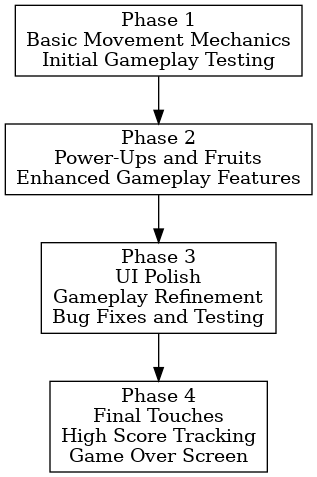
\includegraphics[width=0.3\textwidth]{../Assets/output.png}
    \caption{Development Phases of the Pac-Man Project}
\end{figure}

\end{frame}

\begin{frame}{Progress Update}
    \begin{itemize}
        \item \textbf{Maze Generation:} Implemented (with some debugging needed)
	\item \textbf{Player Movement:} Implemented (with some modifications required)
        \item \textbf{Basic Drawing Functions:} Implemented (walls, pellets, player)
	\item \textbf{Graphics}: Implemented (minute changes left)
    \end{itemize}
\end{frame}

\begin{frame}{Pending Work and Plan for Completion}
    \begin{itemize}
        \item Implementing Pacman's and ghosts' movement and interaction and integrating it in the game loop.
            \begin{itemize}
                \item Implement ghost movement logic and integrate it into the game.
                \item Integrate the Pacman class into the game loop.
                \item Handle collisions between Pacman and ghosts.
		\item Estimated Time: 4-5 days
            \end{itemize}
        
        \item Add additional game mechanics for a complete gameplay experience.
            \begin{itemize}
                \item Creating graphics and adding functionality of power-ups and fruits to the maze.
                \item Implement scoring and life system for multiplayer mode.
		\item Estimated Time: 4-5 days
            \end{itemize}
        
        \item Refine the user interface and graphical elements.
            \begin{itemize}
                \item Design and integrate UI elements (score display, life count, game over screen).
                \item Add animations for Pacman and ghosts.
		\item Estimated Time: 2-3 days
            \end{itemize}
    \end{itemize}
\end{frame}

\begin{frame}{Pending Work and Plan for Completion}
    \begin{itemize}
        \item Integrate Sound Effects
            \begin{itemize}
                \item Add sound effects for eating pellets, power-ups, and ghost interactions.
                \item Integrate background music.
		\item Estimated Time: 2-3 days
	     \end{itemize}
        
        \item Debugging
            \begin{itemize}
                \item Fix any identified bugs or issues.
                \item Optimize performance if needed.
     	    	\item{Estimated Time: 1-3 days}
	    \end{itemize}
    \end{itemize}
  \end{frame}

\begin{frame}{Summary}
    \textbf{Current Status:} The project is progressing well with the basic structure and functionality in place. However, to ensure a complete game consisting of the features planned, additional time is required.
\end{frame}

\begin{frame}
    \centering
    \vfill
    \usebeamerfont{title}\usebeamercolor[fg]{title}\Huge Thank You!
    \vfill
\end{frame}

\end{document}
